% This is a model template for the solutions in computational science. You can find a very useful documentation for LaTeX in Finnish at ftp://ftp.funet.fi/pub/TeX/CTAN/info/lshort/finnish/ or in English at ftp://ftp.funet.fi/pub/TeX/CTAN/info/lshort/english/. The section List of mathematical symbols in Chapter 3 is especially useful for the typesetting of mathematical formulas.

% Compile the document to PDF by command 'pdflatex model.tex' in the terminal. The command must be run twice for the references in the text to be correct.

\documentclass[a4paper,11pt]{article}
\usepackage[utf8]{inputenc}
% This includes letters such as � and �
\usepackage[T1]{fontenc}
% Use here 'Finnish' for Finnish hyphenation. You may have to compile the code twice after the change. 
\usepackage[english]{babel}
\usepackage{graphicx}
% Some math stuff
\usepackage{amsmath,amsfonts,amssymb,amsbsy,commath,booktabs,hyperref}  
% This is just to include the urls
\usepackage{hyperref,subcaption,verbatim}
\usepackage[margin=2cm]{geometry}

\setlength{\parindent}{0mm}
\setlength{\parskip}{1.0\baselineskip}
\usepackage{minted}
\usemintedstyle{tango}

\usepackage{listings}
\usepackage{color}
\usepackage{pdfpages}
\DeclareMathAlphabet{\pazocal}{OMS}{zplm}{m}{n}

\definecolor{dkgreen}{rgb}{0,0.6,0}
\definecolor{gray}{rgb}{0.5,0.5,0.5}
\definecolor{mauve}{rgb}{0.58,0,0.82}

\lstset{frame=tb,
	language=Python,
	aboveskip=3mm,
	belowskip=3mm,
	showstringspaces=false,
	columns=flexible,
	basicstyle={\tiny\ttfamily},
	numbers=none,
	numberstyle=\tiny\color{gray},
	keywordstyle=\color{blue},
	commentstyle=\color{dkgreen},
	stringstyle=\color{mauve},
	breaklines=true,
	breakatwhitespace=true,
	tabsize=4
}

\begin{document}

\title{CS-E4830 Kernel Methods in Machine Learning \\ Assignment 2} % Replace the exercise round number
\author{Kunal Ghosh, 546247} % Replace with your name and student number
\maketitle
\section*{}
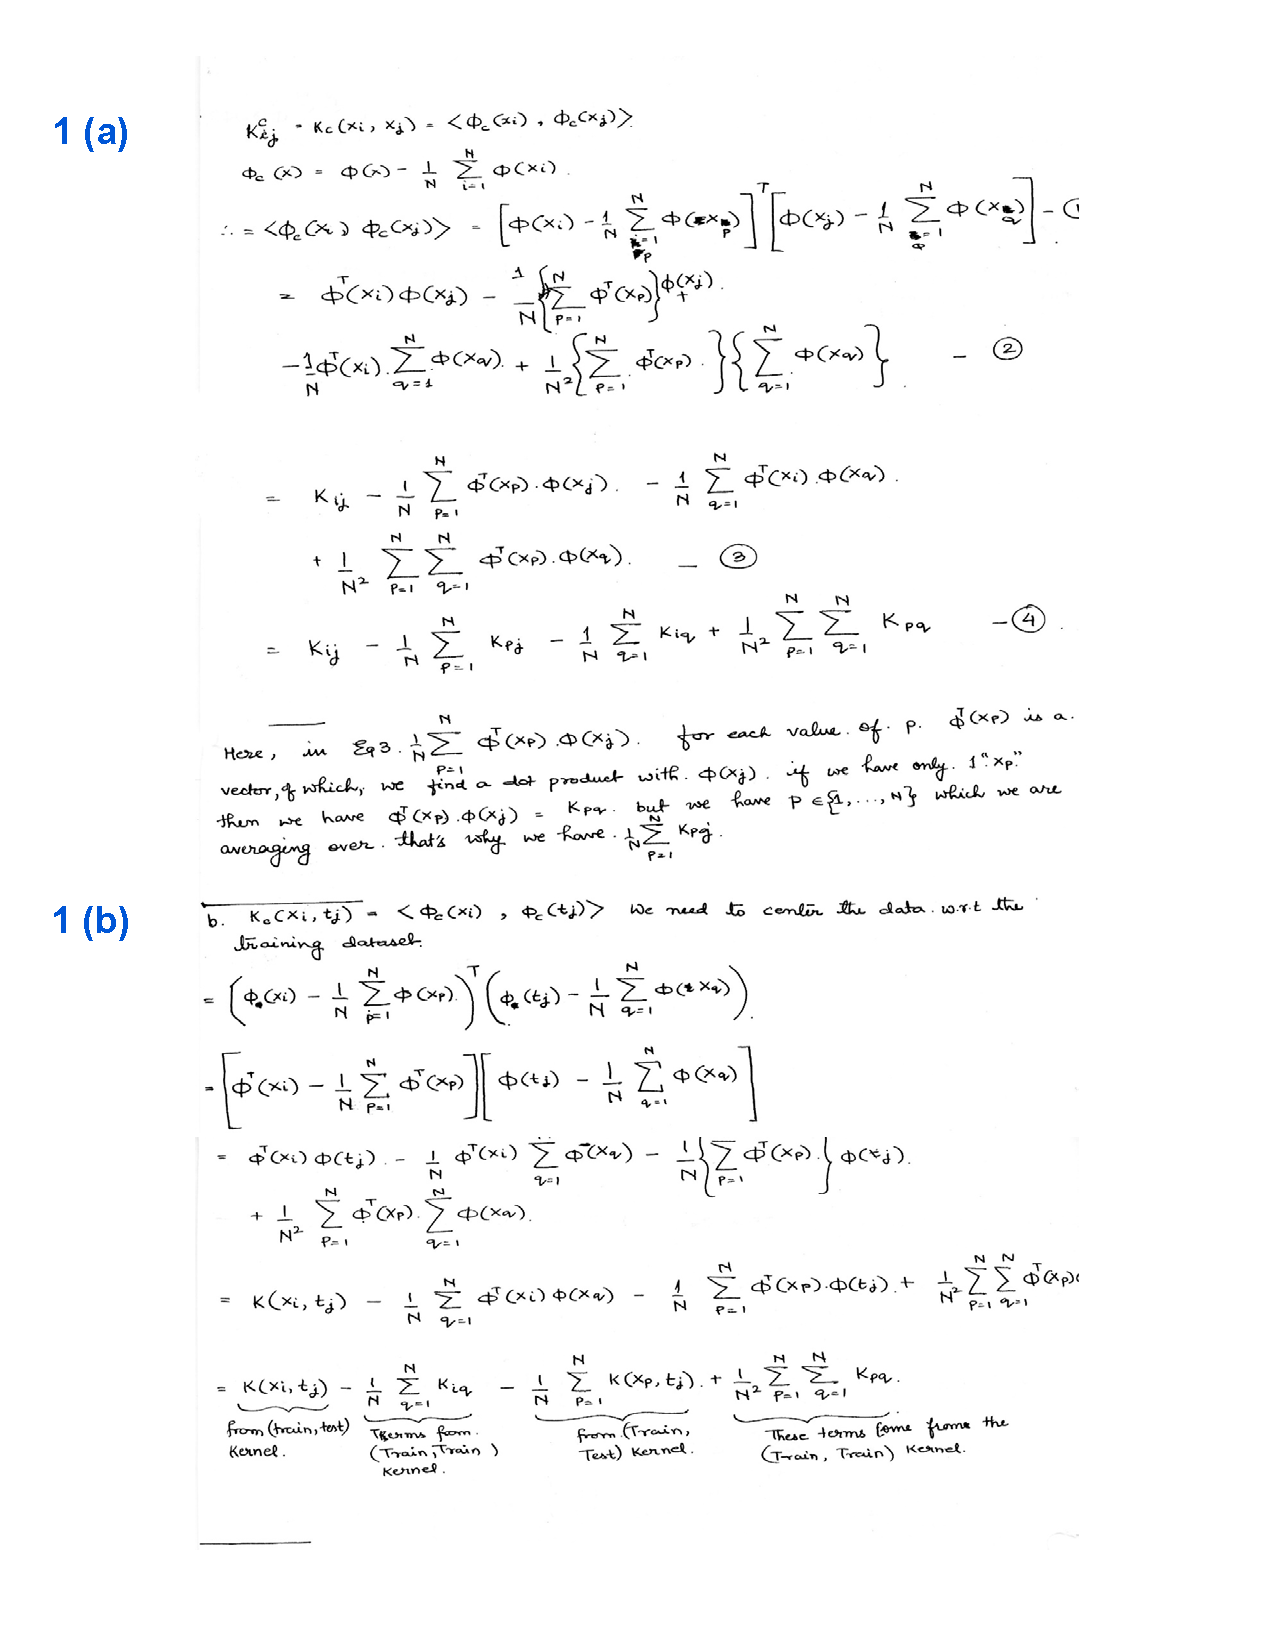
\includepdf[pages=-]{q1n2-3.pdf}
\section*{Solution to Question 3}
\inputminted[baselinestretch=1, fontsize=\small, breaklines=true]{octave}{../kernel_ridge_regression.m}
\section*{Solution to Question 4}
\inputminted[baselinestretch=1, fontsize=\small, breaklines=true]{octave}{../get_prediction_mse.m}

We can then encapsulate the \texttt{kernel\_ridge\_regression} method and the \texttt{get\_prediction\_mse} method to a more convenient single method. 

\inputminted[baselinestretch=1, fontsize=\small, breaklines=true]{octave}{../kernel_ridge_regression_on_dataset.m}
\section*{Solution to Question 5 (a)}
Applying the \texttt{kernel\_ridge\_regression} code to the UCI forest fire dataset.
\inputminted[baselinestretch=1, fontsize=\small, breaklines=true]{octave}{../forest_fire_predict_new.m}
\begin{figure}[ht]
    \centering
    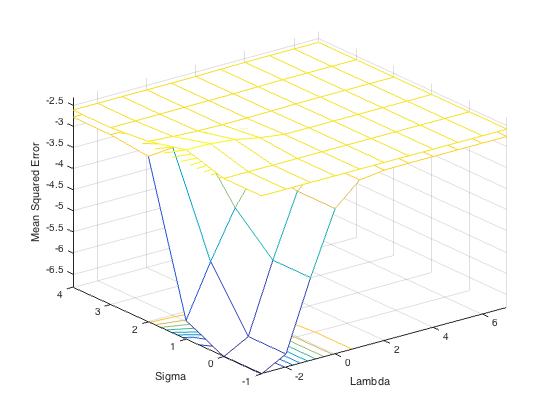
\includegraphics[width=1.1\linewidth]{../3d.png}
    \label{fig:mse}
    \caption{\textit{MSE of Test data (top plane) and Training data (bottom plane)} \textbf{all values in log10 scale}. \\In the plot above, for \textit{sigma} values between $10^{-1} \text{ and } 10^{2}$ and \textit{lambda} values between $10^{-3} \text{ and } 1$ \textit{(all pairs)} we notice that the training error (bottom plane) is much lower than the test error (top plane). This would imply that for these values of sigma and lambda the model is overfitting to the training dataset. However, for rest of the values of sigma and lambda the training and test errors don't have a huge gap so we can say that for those parameter values the model generalizes well.\\\textbf{Observation:} In the above plot, for a small sigma and lambda values, we see that there is overfitting. But for any given (small) sigma, as we increase the regularization (lambda increased) the overfitting reduces and that's as expected. However, for larger sigma values there is no overfitting even for small regularization and so, increasing the regularization doesn't have any effect. }
\end{figure}
\section*{Solution to Question 5 Part (b)}
Parameter combination with lowest cross-validation error. Also reported is the mean-squared-error on the test set using the parameter combination. Note that we have not retrained the model using the best sigma and lambda values since we had already calculated and saved the MSE values for all sigma and lambda pairs. We have just reported the saved MSE values for the best (cross-validated) parameters which should remain same when the model is trained again using these parameters. 

\begin{verbatim}
mse_test_for_best_params =

    0.0031

best_sigma =

    10

best_lambda =

     1
\end{verbatim}
\subsubsection*{Code to compute the \textit{k-fold} cross-validation error}
The function below is being invoked in the script defined in \texttt{Solution to Question 5 part (a)}
\inputminted[baselinestretch=1, fontsize=\small, breaklines=true]{octave}{../get_k_fold_cv_error_new.m}
\end{document}

   

